\documentclass{article}
\usepackage[UTF8]{ctex}
\usepackage{pythonhighlight}

% Language setting
% Replace `english' with e.g. `spanish' to change the document language
\usepackage[english]{babel}
\usepackage{float}
% Set page size and margins
% Replace `letterpaper' with `a4paper' for UK/EU standard size
\usepackage[letterpaper,top=2cm,bottom=2cm,left=3cm,right=3cm,marginparwidth=1.75cm]{geometry}

% Useful packages
\usepackage{amsmath}
\usepackage{graphicx}
\usepackage[colorlinks=true, allcolors=blue]{hyperref}

\title{进度汇报2}
\author{雷远航}

\begin{document}

\maketitle

\begin{abstract}
第二次进度汇报

\end{abstract}

\section*{一:知识学习和总结}
本阶段我主要学习了Chapter7 Feature detection and matching,在这一章中有许多新的概念,并且介绍了很多
检测与匹配的算法,由于书中有很多之前未接触过的术语,以及很多新的内容的介绍,所以在理论部分的学习花费了比较大的精力.

通过这一阶段的学习我主要理解体会了:点检测和线检测这两种主要的方法,以及相应的算法原理,书中的一些算法只是一些介绍性质的,我尽我所能的对我进行测试的算法进行了理论上的理解,通过使用opencv的练习完成了对一些算法的
detectors->desciptors->matching的过程,但有一些算法如果真正实现起来对我来说还有一定的困难,在练习时我只是调用了相应的函数接口来完成.

\section*{二:一些提问}

1.我在进行一些图像的测试时如果图像有一些较强的光线的干扰时会对图像的特征点以及匹配时造成一些
误判,产生错误的匹配.在实际的研究当中,在进行图像匹配时,这种光线强度的因素是否是一个较大的干扰?

2.对于图像匹配的问题,我看到也有很多利用深度学习来获取图像的特征以及进行匹配的方法,目前基于深度学习的匹配算法的应用如何?



\section*{三:练习}

\subsection*{Harris算法:}
利用Harris算法进行角点检测
    \begin{figure}[H]
    \centering
    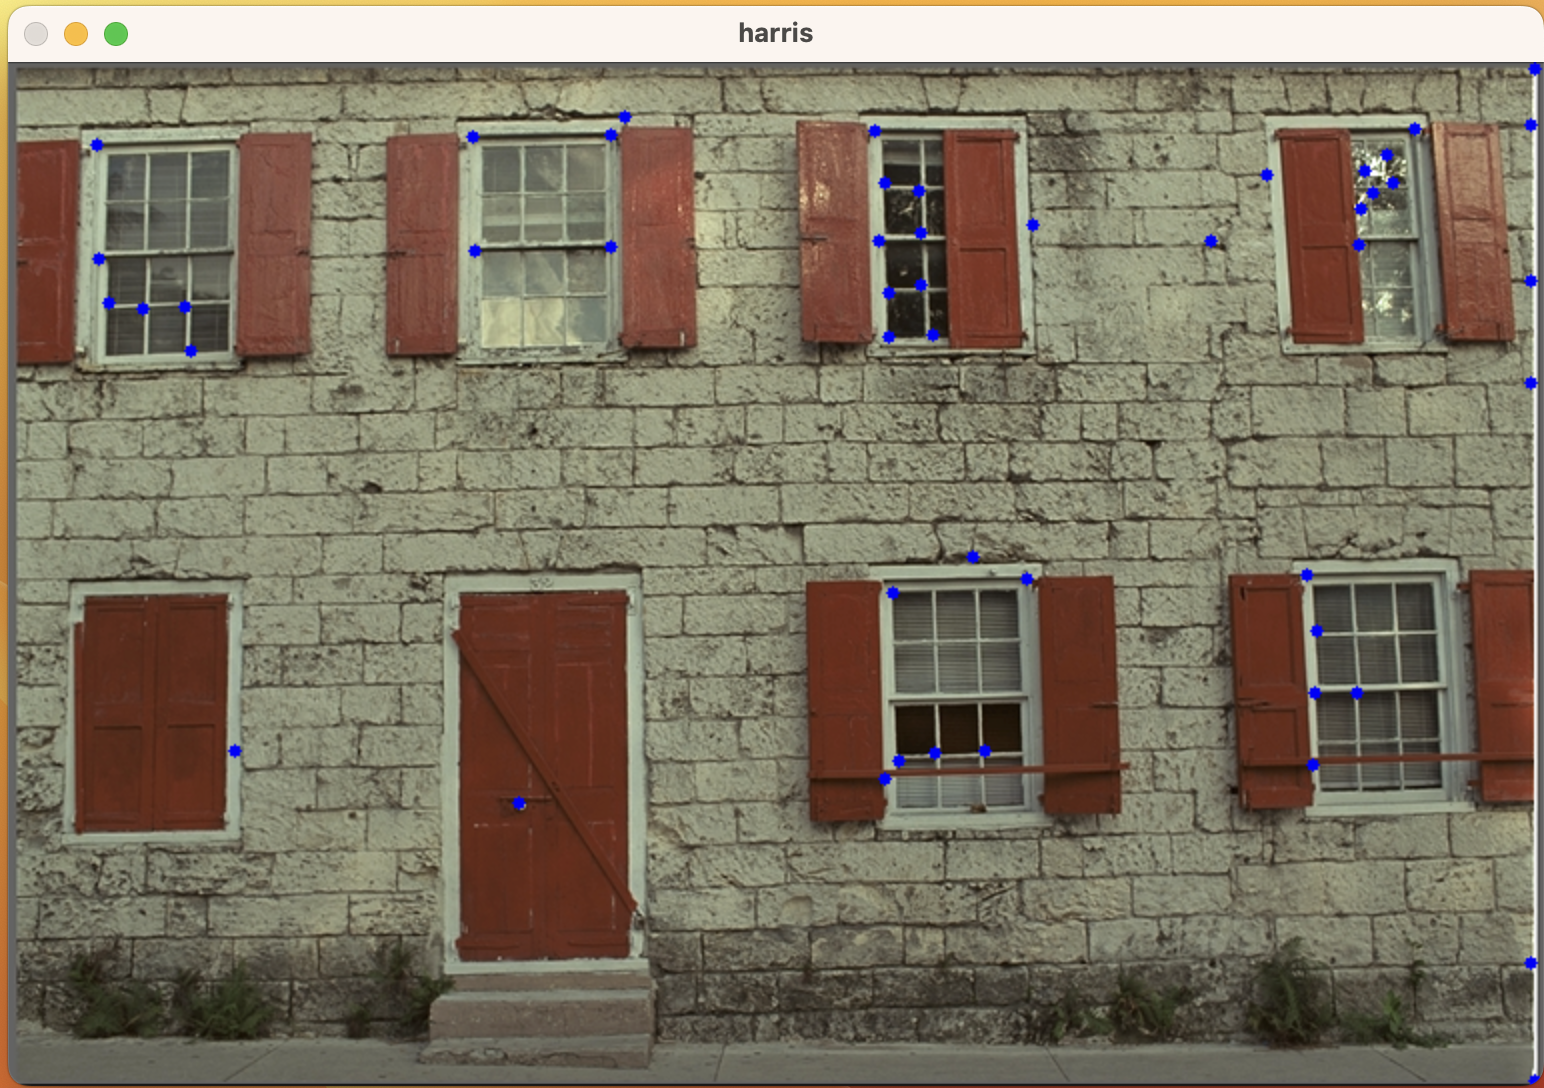
\includegraphics[width=0.8\textwidth]{1.png}
    \caption{\label{pr2}Harris算法}
    \end{figure}



\subsection*{SIFT检测器:}
\begin{figure}[H]
    \centering
    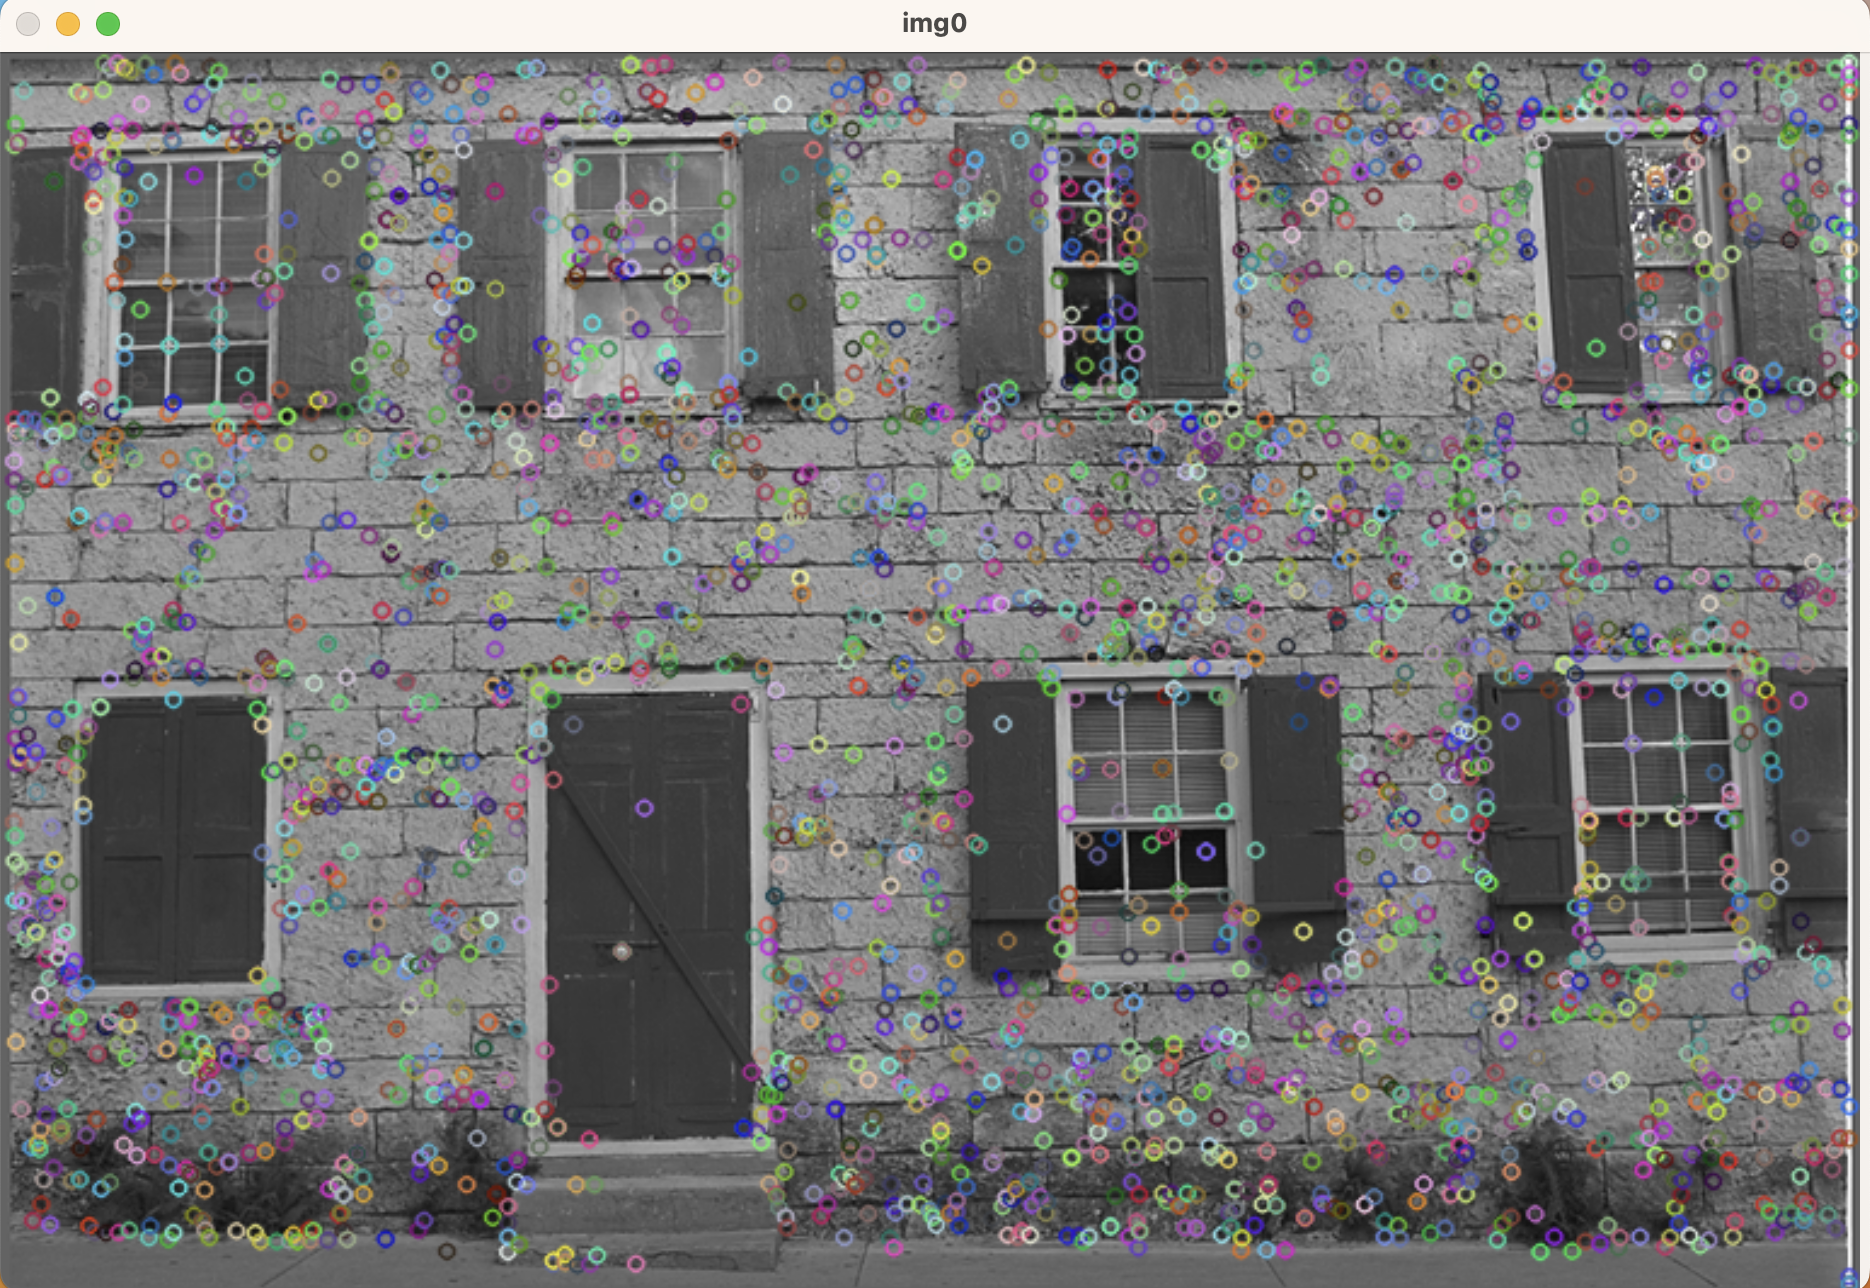
\includegraphics[width=0.8\textwidth]{2.png}
    \caption{\label{pr2}SIFT算法}
    \end{figure}

\subsection*{ORB检测器:}
    \begin{figure}[H]
        \centering
        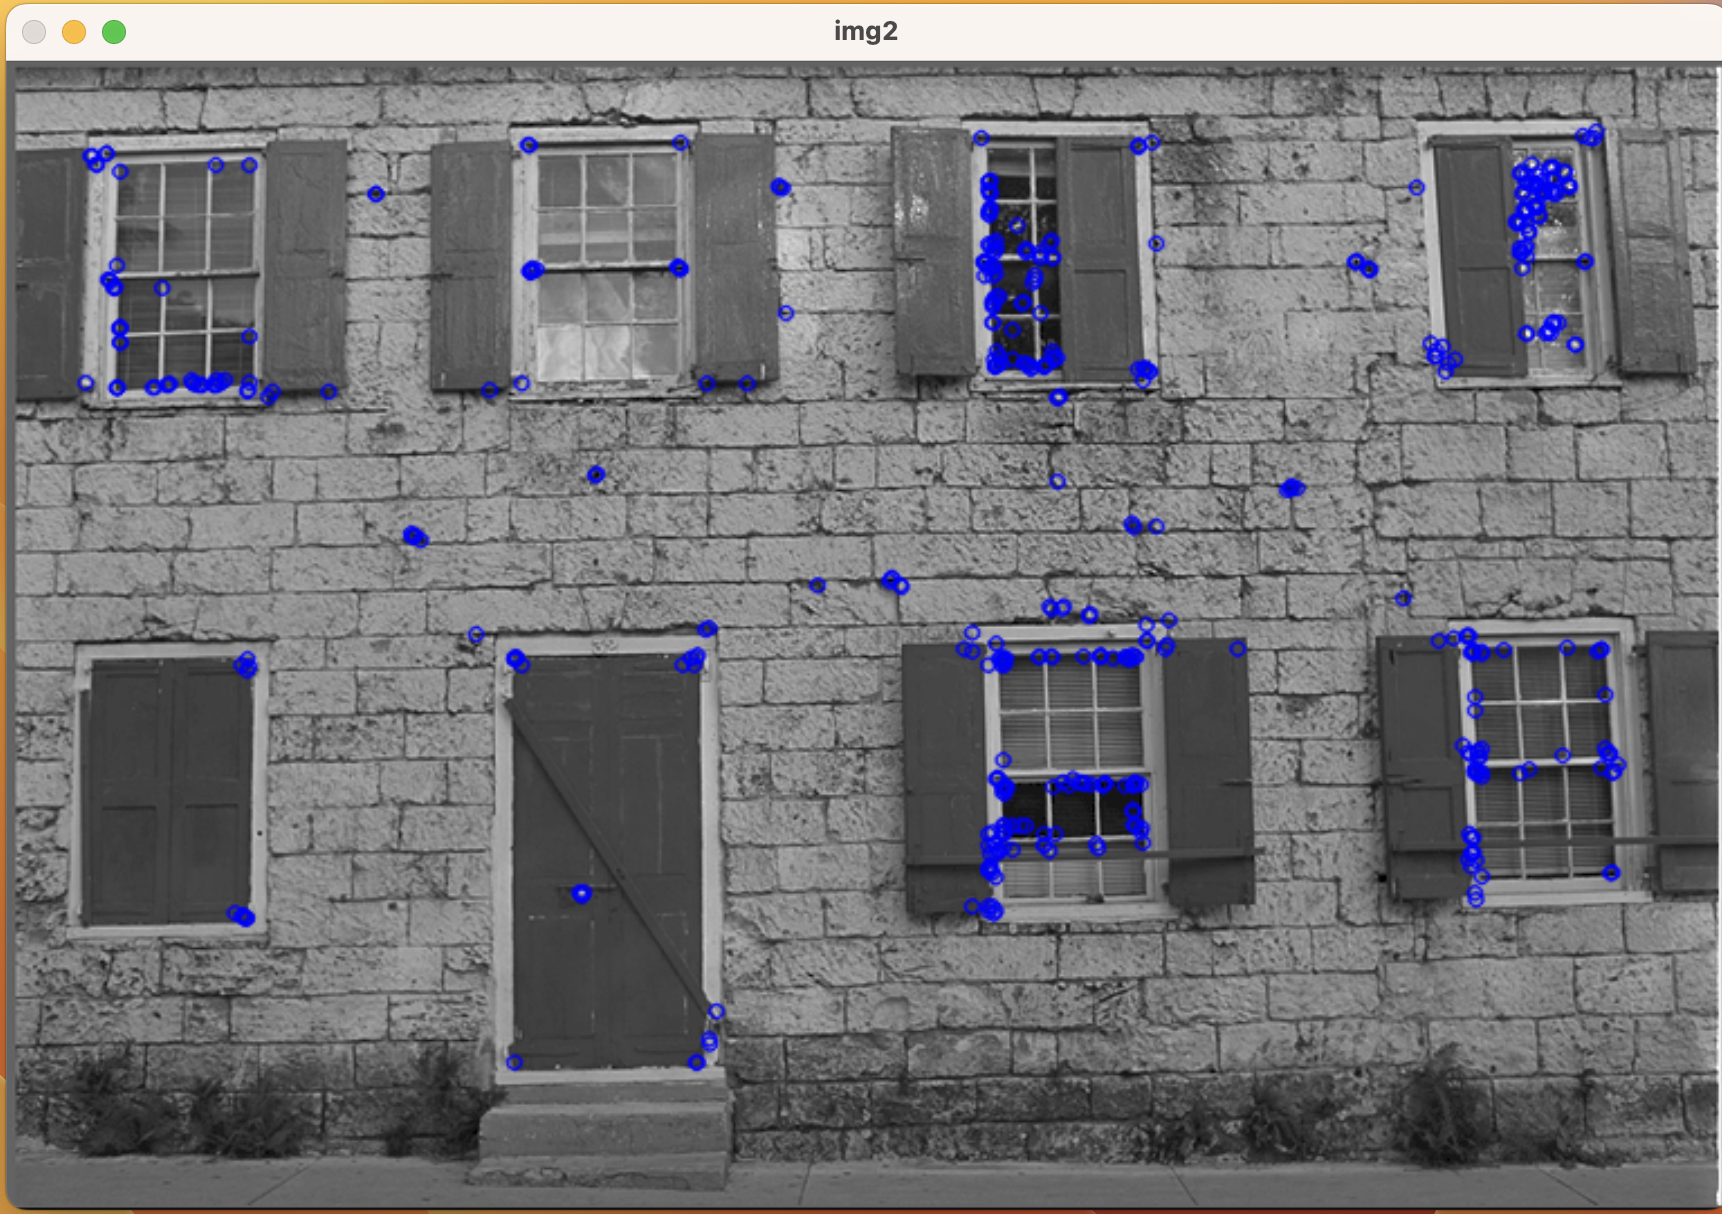
\includegraphics[width=0.8\textwidth]{3.png}
        \caption{\label{pr2}ORB}
        \end{figure}

\subsection*{Hough算法}
利用Hough算法对线边缘进行检测
\begin{figure}[H]
    \centering
    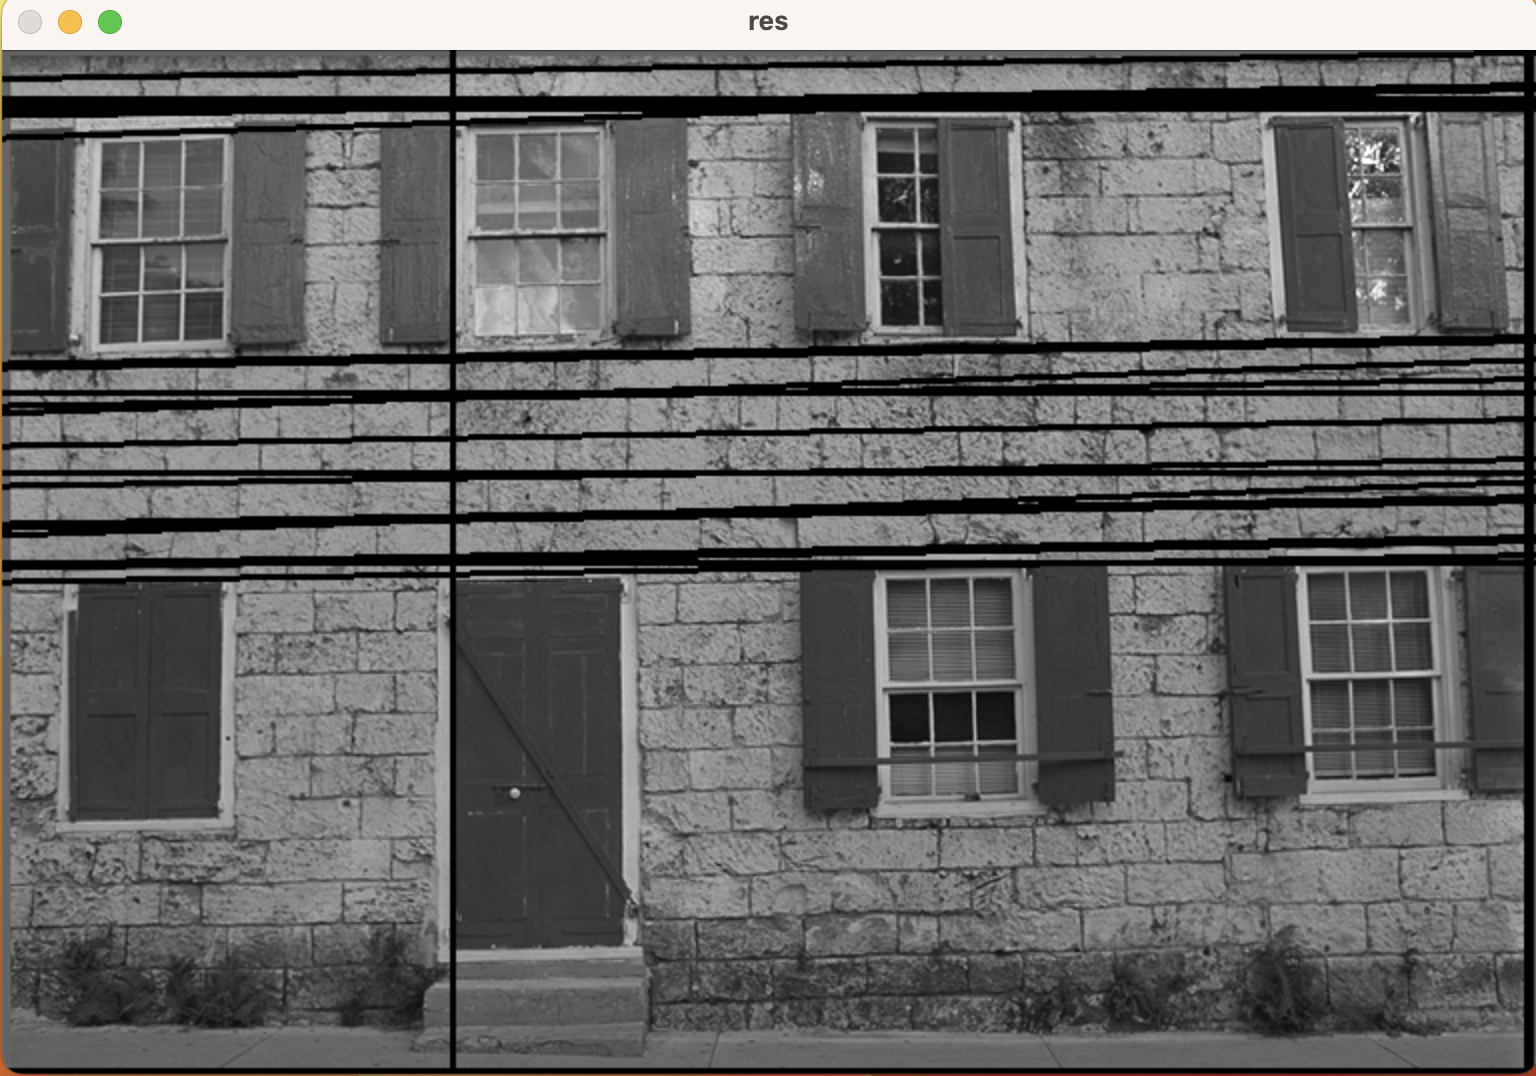
\includegraphics[width=0.8\textwidth]{4.png}
    \caption{\label{pr2}Hough}
    \end{figure}

    \begin{figure}[H]
        \centering
        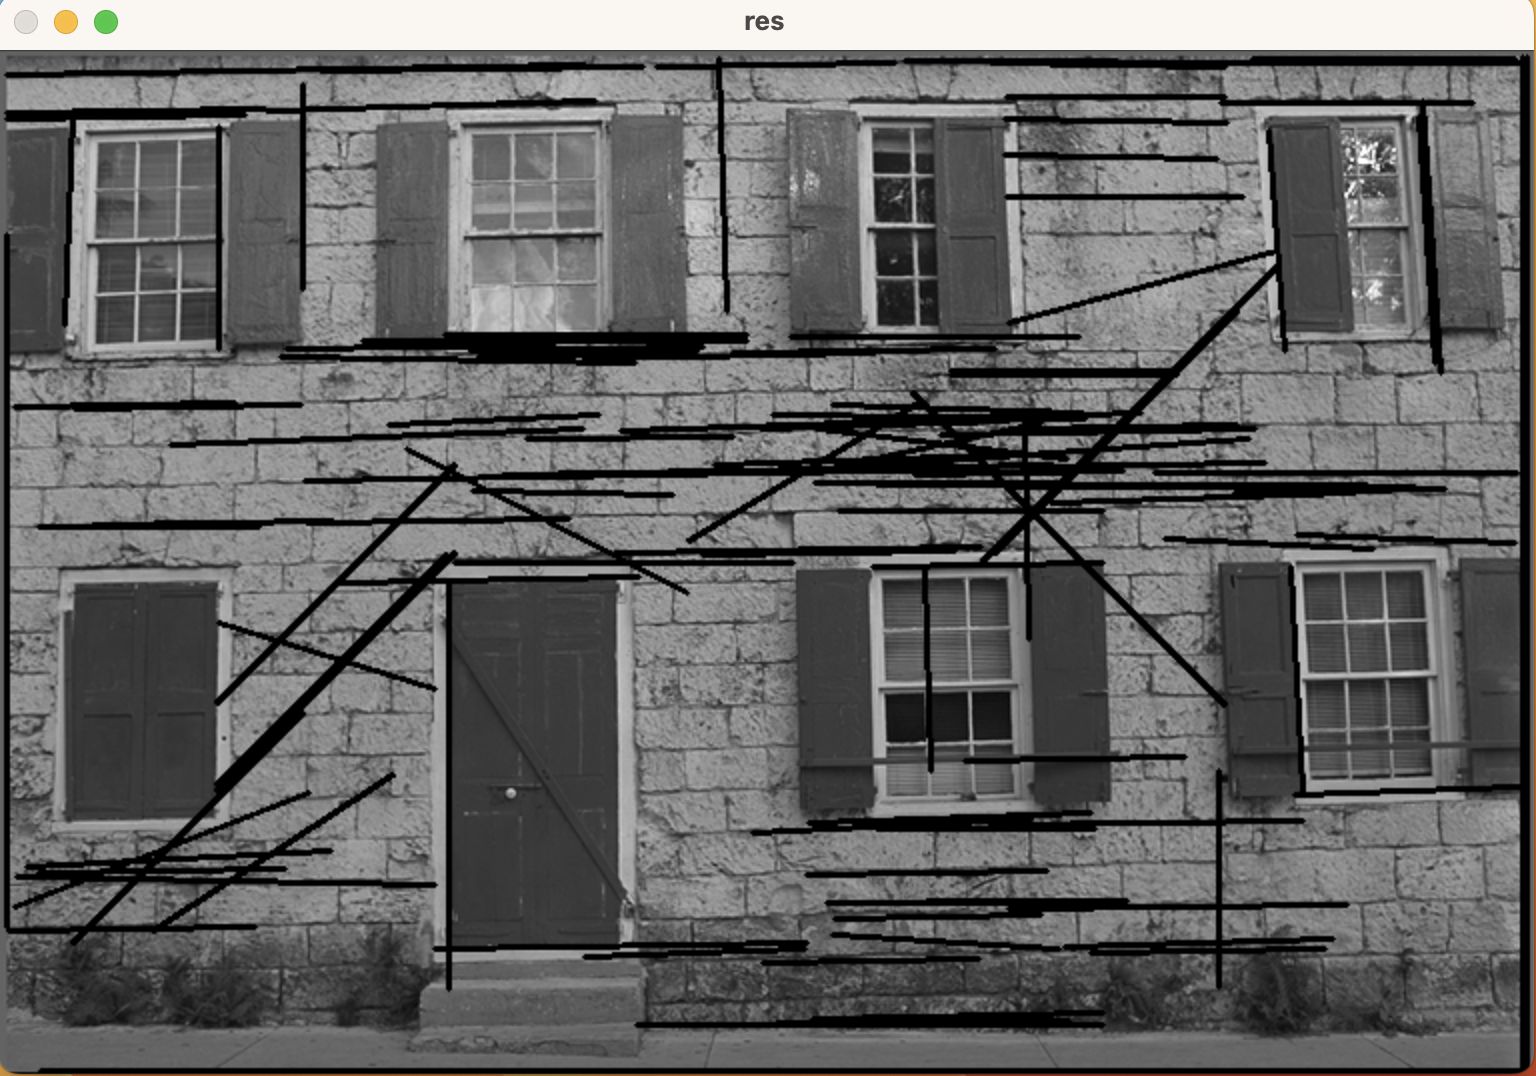
\includegraphics[width=0.8\textwidth]{5.png}
        \caption{\label{pr2}Match}
        \end{figure}

\subsection*{SIFT+Brute-Force匹配 }
在我使用实际拍摄的图片进行测试时,这个算法可以进行很好的匹配
\begin{figure}[H]
    \centering
    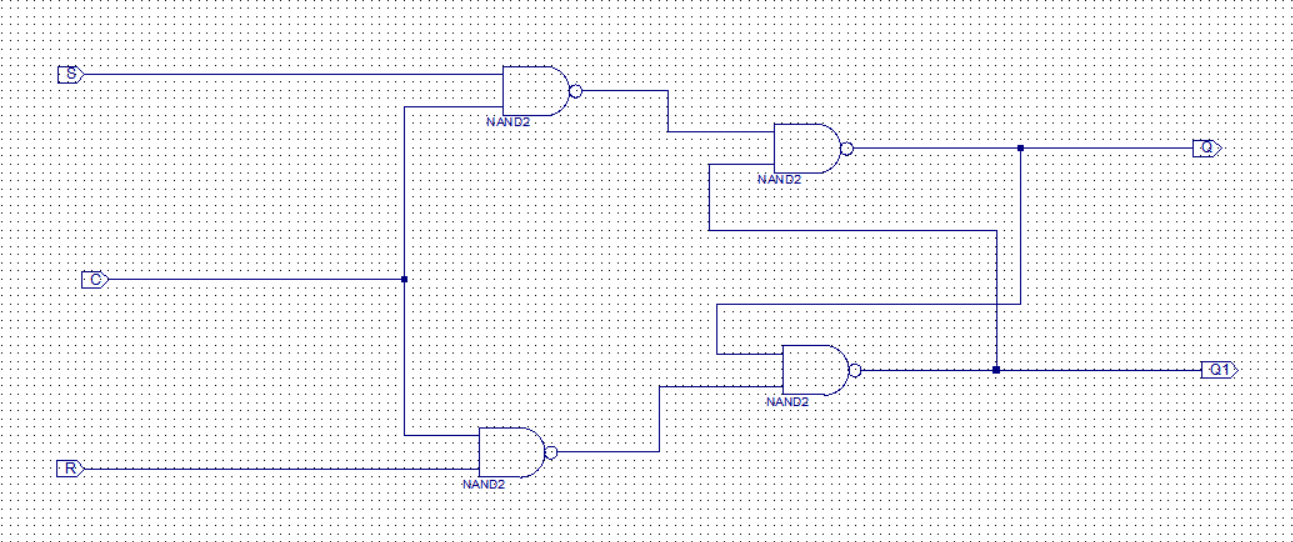
\includegraphics[width=0.8\textwidth]{6.png}
    \caption{\label{pr2}Match}
    \end{figure}

\subsection*{ORB+Brute-Force匹配}

在匹配时如果周围的干扰比较小可以正确匹配.
\begin{figure}[H]
    \centering
    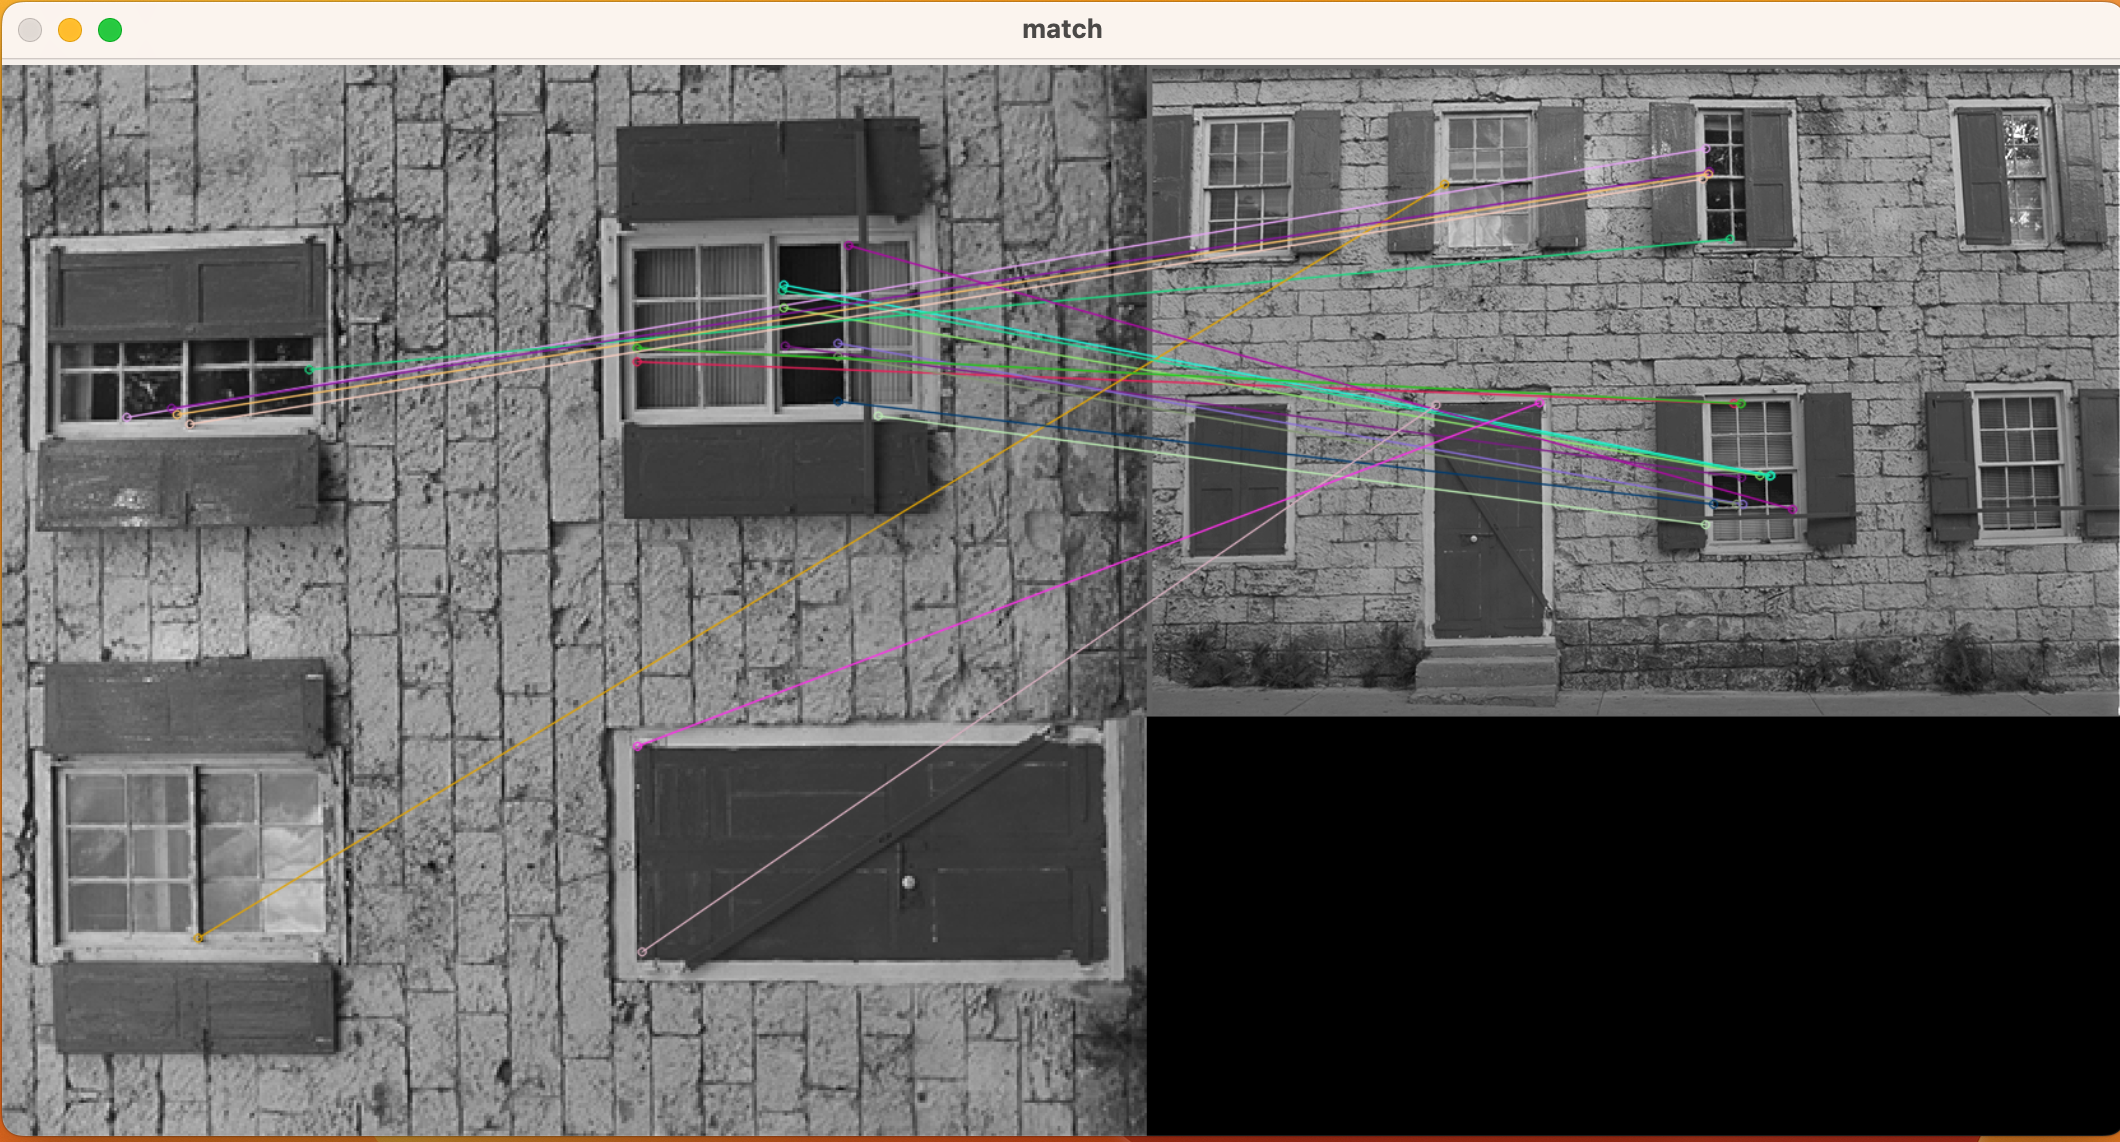
\includegraphics[width=0.8\textwidth]{8.png}
    \caption{\label{pr2}Match}
    \end{figure}

这个算法匹配失败的例子
\begin{figure}[H]
    \centering
    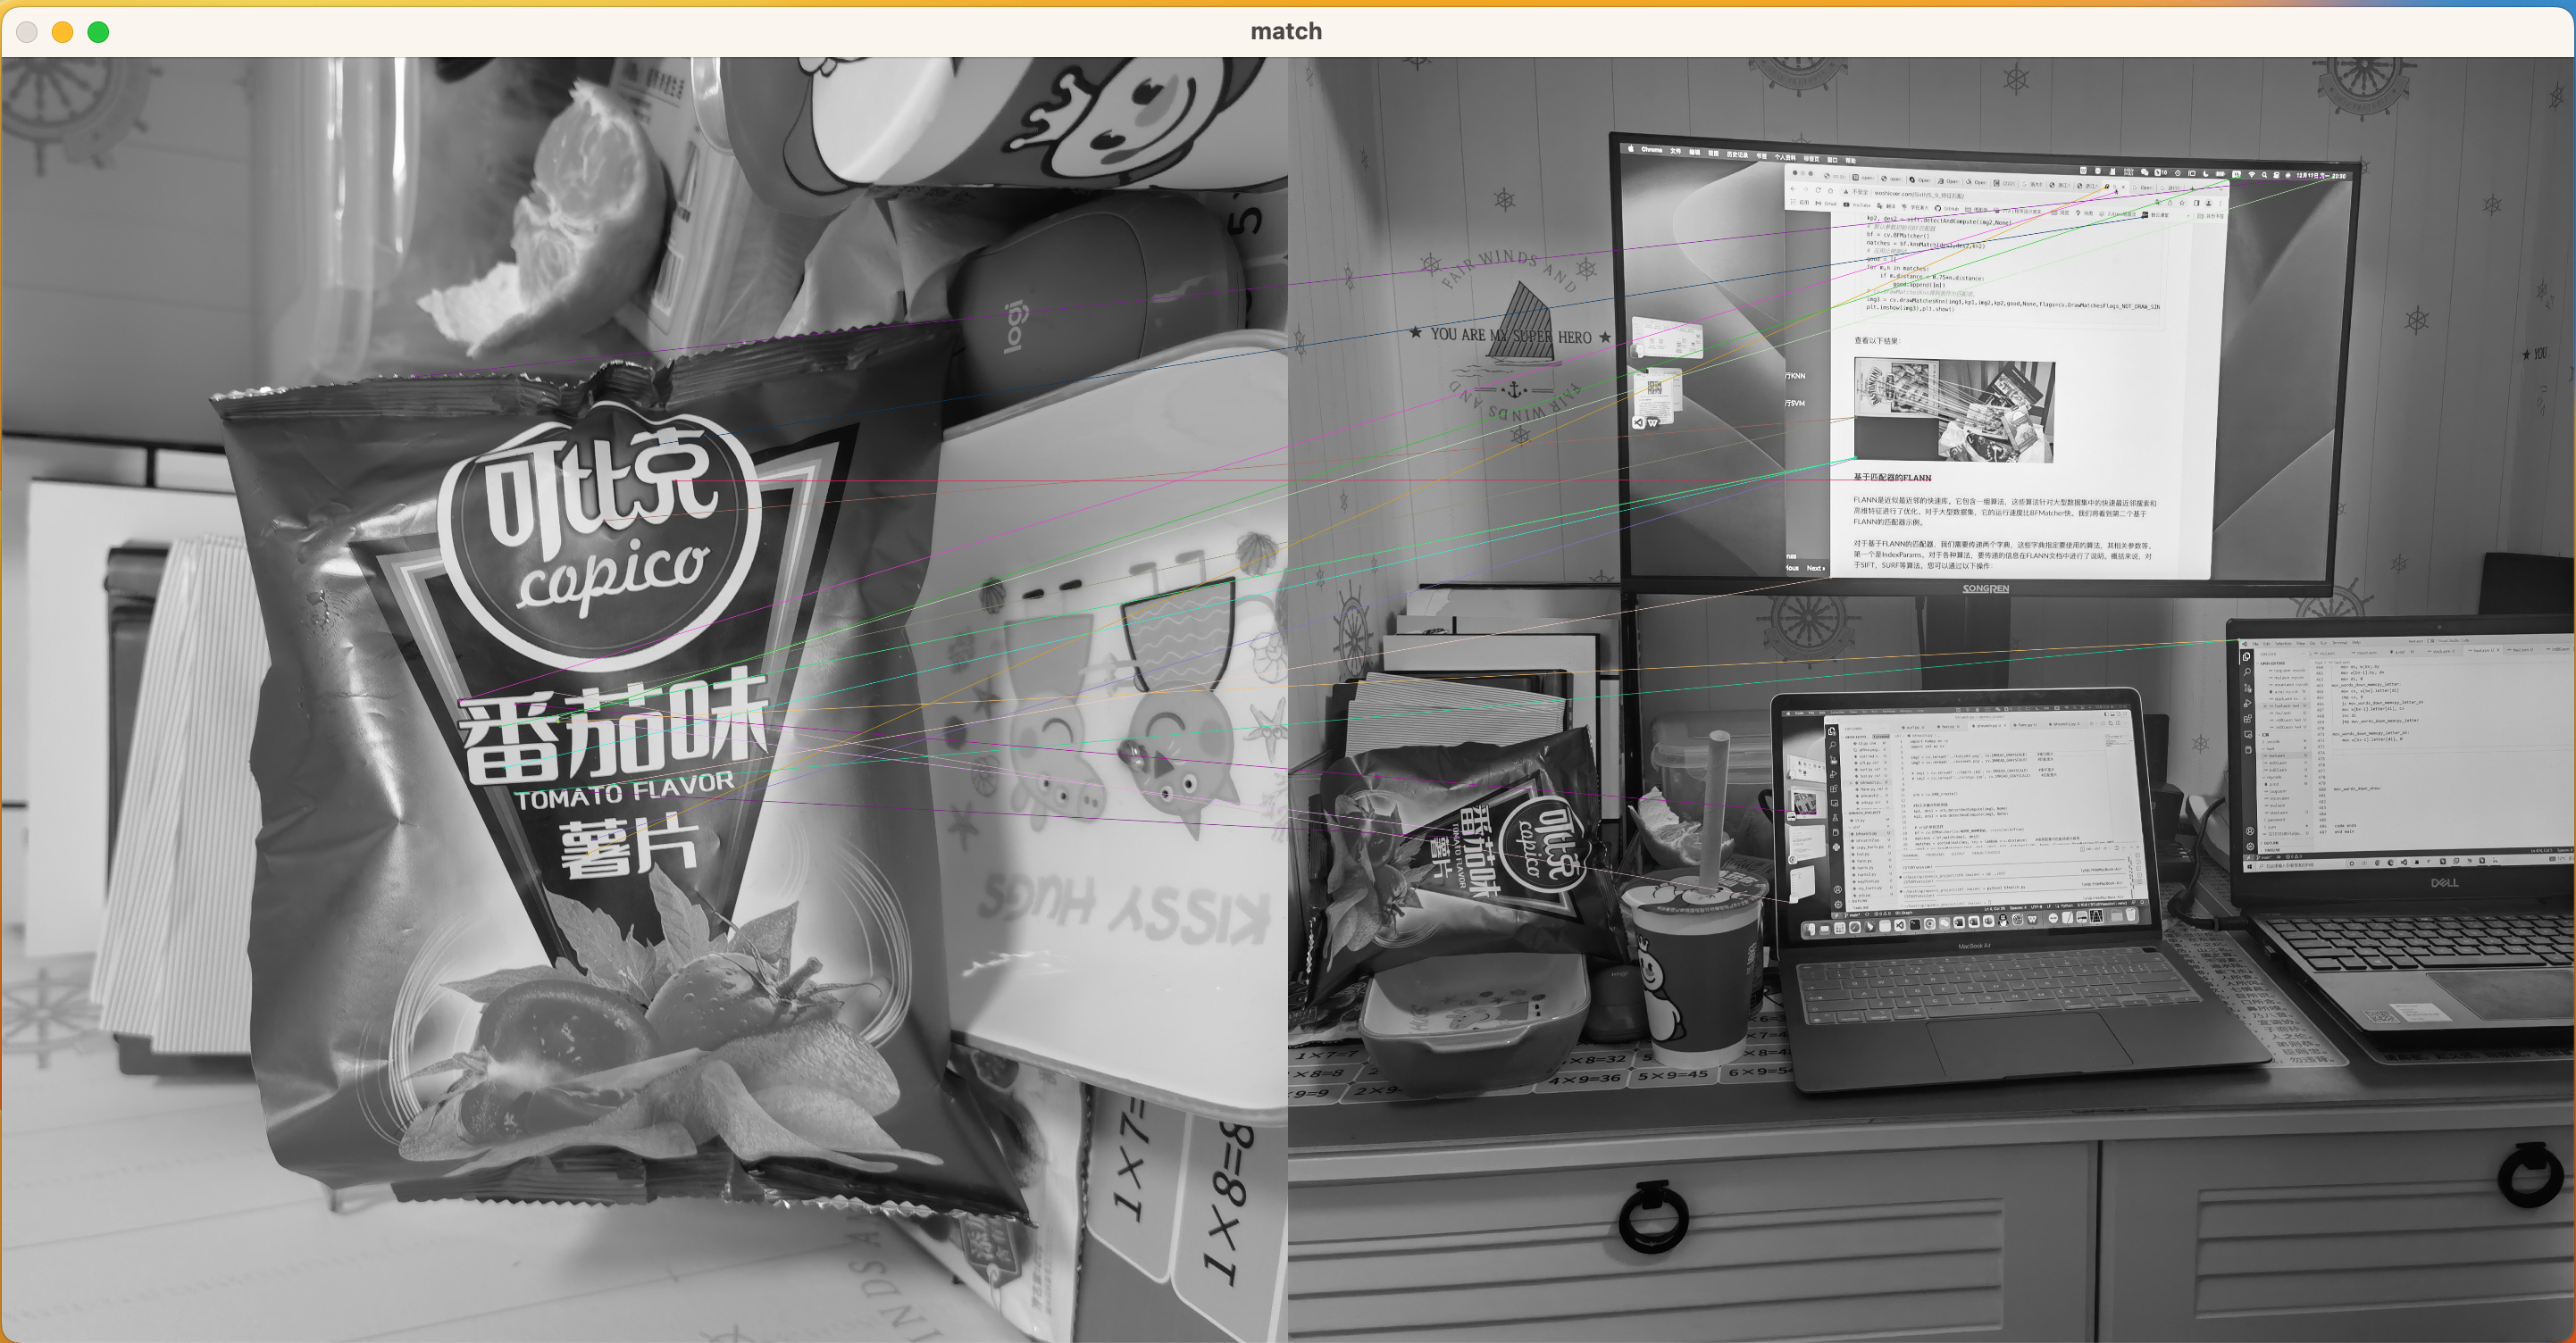
\includegraphics[width=0.8\textwidth]{7.png}
    \caption{\label{pr2}Match}
    \end{figure}


\subsection*{SIFT+FLANN匹配}
\begin{figure}[H]
    \centering
    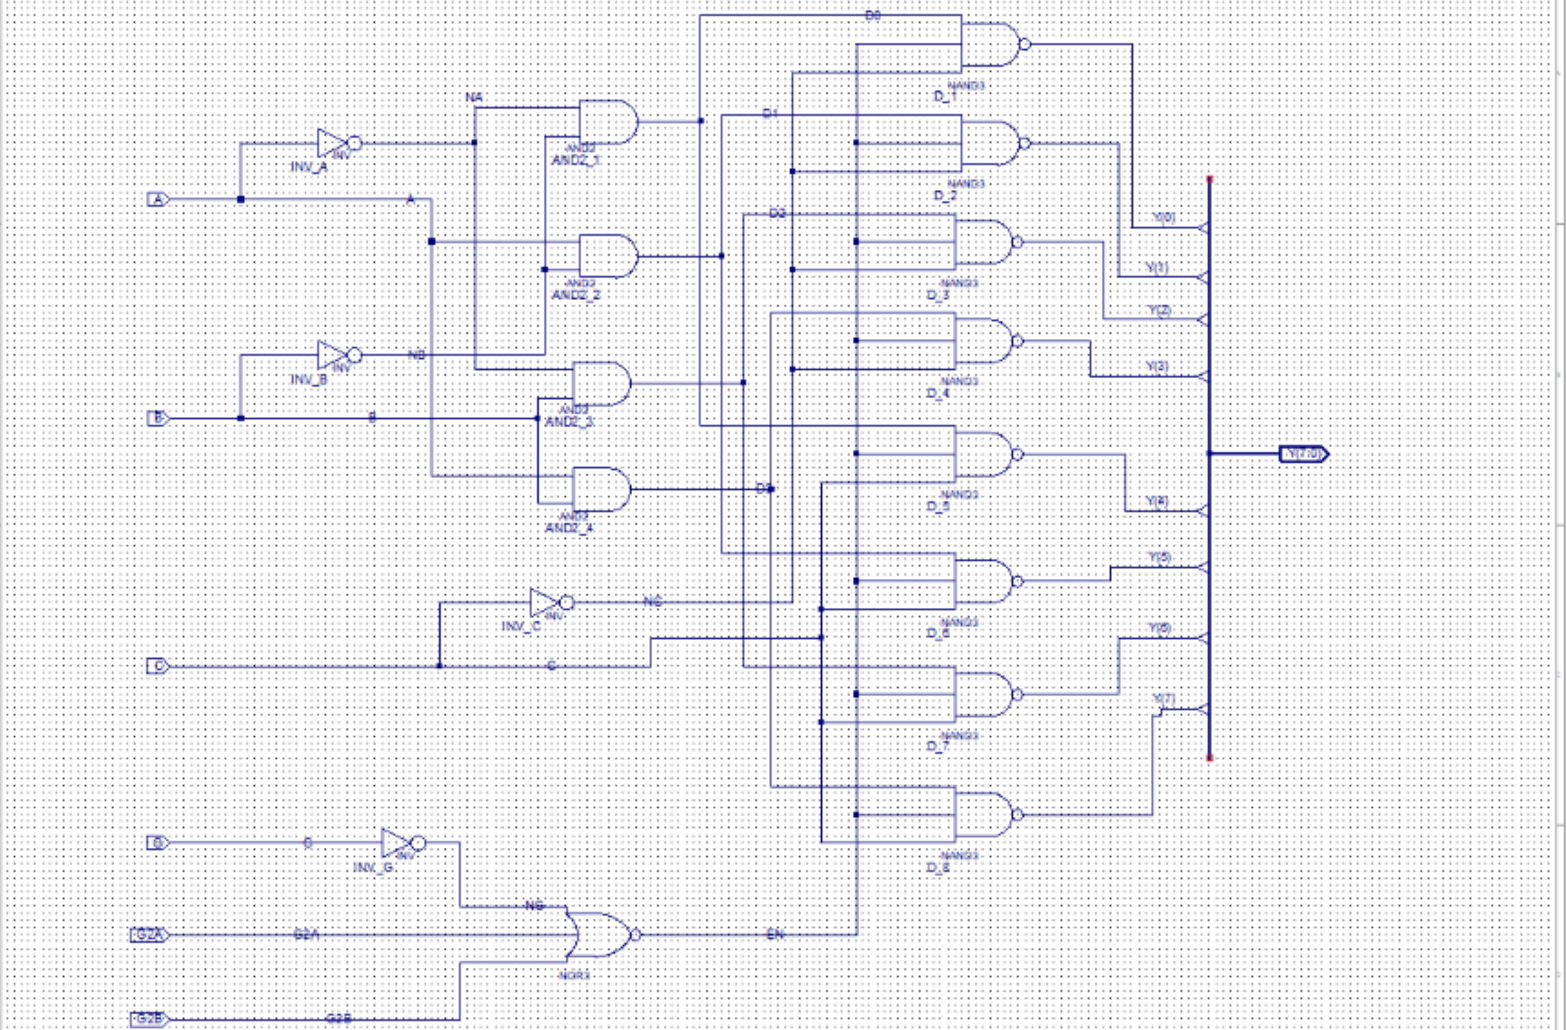
\includegraphics[width=0.8\textwidth]{9.png}
    \caption{\label{pr2}Match}
    \end{figure}


\end{document}